\chapter{Algorithm description}

This chapter describes the obstacle detection algorithm: First a short description of the input data and the assumptions made throughout the algorithm are given. Then the two major stages of the algorithm are presented: \textit{Depth reconstruction} and the actual \textit{obstacle detection}. While the first stage aims at reconstructing the world position of each pixel by implicitly calculating optical flow between two sequentially captured images, the second stage refines these results by accumulating the uncertainty distributions of the reconstructed landmark points obtained from multiple depth reconstruction steps in a local environment map.

\section{Prerequisites}

This section covers both a description of the input data and a list of assumptions that are (sometimes implicitly) made throughout the following sections.

\subsection{Input data: motion parameters and panoramic images}

\begin{figure}[htb]
 \begin{center}
  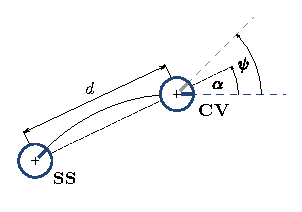
\includegraphics[width=0.5\textwidth]{media/robot_relative_movement.pdf}
 \end{center}
 \caption{Description of the motion parameters $d, \alpha, \psi$. The two circles depict the robot position and orientation (blue angle marks) under which the snapshot $\img{SS}$ and current view $\img{CV}$ were captured. The actual robot trajectory (solid line) is not required as the motion is fully described by the translatory distance $d$, the movement direction $\alpha$ and the change in orientation expressed by $\psi$.}
 \label{fig:robot_relative_movement}
\end{figure}

\begin{figure}[tbp]
  \begin{center}
   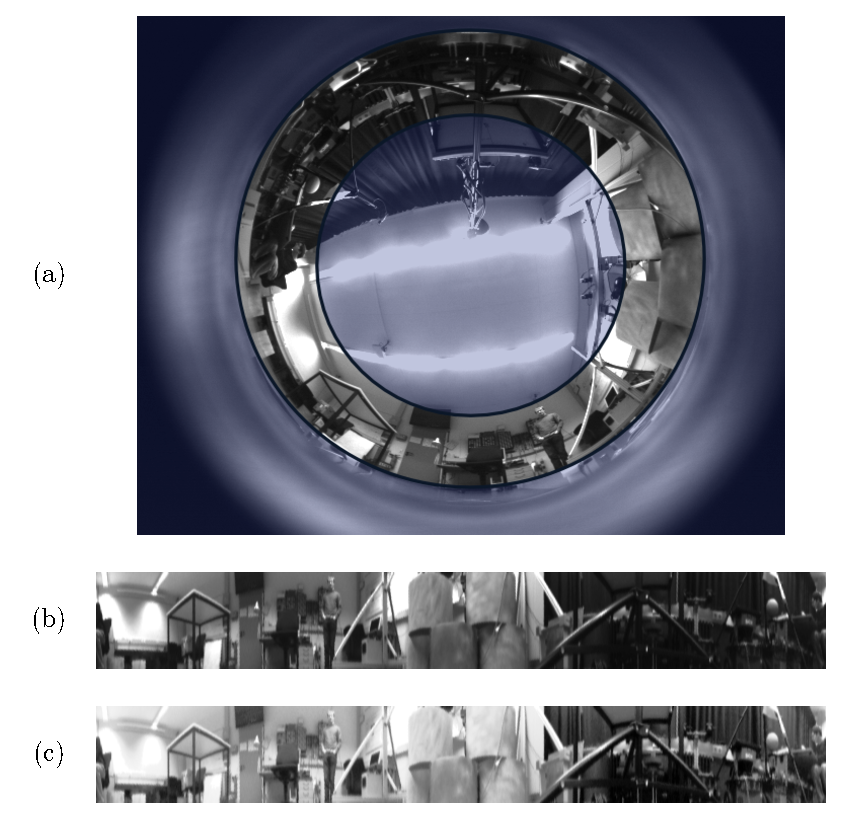
\includegraphics[scale=0.65]{media/cylindrical_panoramic_images_unprojected_pix.pdf}
  \end{center}
  \caption{(a) The original $640 \times 512$ pixel frame as recorded by the camera. The region used for the panoramic image is highlighted, with the outer circle being the bottom row in the result images (specified by the \textit{depression} angle $\check \gamma$) and the inner circle being the top row in the result images (specified by the \textit{elevation} angle $\hat \gamma$). (b) The unrolled $720 \times 96$ pixel cylindrical panoramic image. (c) Cylindrical image after applying histogram equalization.}
  \label{fig:cylindrical_panoramic_images_unprojected}
\end{figure}

The input of the obstacle detection algorithm is given as a pair of monochrome panoramic images, denoted $\img{SS}$ and $\img{CV}$ (snapshot and current view), accompanied by a set of motion parameters $d, \alpha$ and $\psi$.

\paragraph{Motion parameters:} As depicted in figure \ref{fig:robot_relative_movement} the motion parameters $d, \alpha$ and $\psi$ describe a motion vector leading from the snapshot position to the current view position. The Euclidean distance in meters is denoted by $d$, whereas the motion direction is denoted by the angle $\alpha$. The change in orientation under which the two images were captured is denoted by $\psi$.

\paragraph{Panoramic images:}
\label{sec:panoramic_image}
The fisheye images as captured from the camera are not directly used in the algorithm. As discussed in the introduction (section \ref{sec:intro_special}), the actual region of interest is too small to justify the usage of the complete input image. Instead the interesting region is mapped (using a lookup table that is generated in a calibration process) to a spherical panoramic image. The source region is chosen larger than the region of interest, as this extension will later (see section \ref{sec:memory_layout}) be needed for pixel lookups. Additionally, histogram equalization is applied to the images in order to increase the contrast and to compensate global illumination changes. See figure \ref{fig:cylindrical_panoramic_images_unprojected} for an example. This and the following chapters assume such a spherical panoramic image and are independent of the actual image source.

\paragraph{Panoramic image coordinate system:}
\label{sec:panoramic_coordinates}
The panoramic images contain a $360^\circ$ view of the surroundings such that the $x$-, $y$-pixel coordinates of the image linearly correspond to a pair of angles $\beta, \gamma$ which --- in conjunction with the yet unknown landmark distance $r$ --- describe the position of the projected landmark in spherical coordinates (note that an elevation angle of $\gamma = 0$ corresponds to the image horizon and not the zenith). Let $w, h$ denote the image width and height. It holds:
\begin{align*}
 \beta(x) &= \frac{2 \pi}w \cdot x & \gamma(y) &= \frac{\check \gamma - \hat \gamma}{h - 1} \cdot y + \hat \gamma
\end{align*}
where $\check \gamma$ is the so called \textit{depression} describing the elevation angle of the bottom image row and $\hat \gamma$ the so called \textit{elevation} describing the elevation angle of the top image row. The angles $\beta$ and $\gamma$ respectively correspond to azimuthal component and polar component of spherical coordinates (see figure \ref{fig:cylinder_coordinates_simple} for an illustration).

In contrast to classical spherical coordinates, the distance $r = \tilde r \cdot \cos(\gamma)$ (with $\tilde r$ being the Euclidean distance) is measured as ground distance, which will allow for simplified equations and the separability of the motion field equation, as discussed in section \ref{sec:flow_template_calculation}. As depicted in figure \ref{fig:hypot_vs_ground_distance}, the change in the measurement of $r$ only effects the representation of a series of equal-distanced landmarks. Moreover, points with an elevation angle of $\gamma = \pm 90^\circ$ cannot be uniquely described in this coordinate system.

Because $\beta, \gamma$ and the pixel coordinates $x, y$ can be used synonymously, the individual intensity values of an image $\img{I}$\footnote{A note on notation: Two-dimensional fields $\img{I}$ of scalars or low dimensional vectors (images, depth maps, index maps) are denoted in bold letters. This is not true for ``small'' matrices (convolution kernels), fields of functions or fields of sets.} are subsequently denoted by $\img{I}(\vec p) = \img{I}(\beta, \gamma)$. As the panoramic images are cyclic in horizontal direction, arbitrary $\beta$ values are cyclically mapped onto the interval $[0, 2\pi)$. If the pixel coordinates $x, y$ corresponding to a $\beta, \gamma$ pair are non-integral, bilinear interpolation between the neighboring pixels is applied.

\begin{figure}[p]
  \begin{center}
   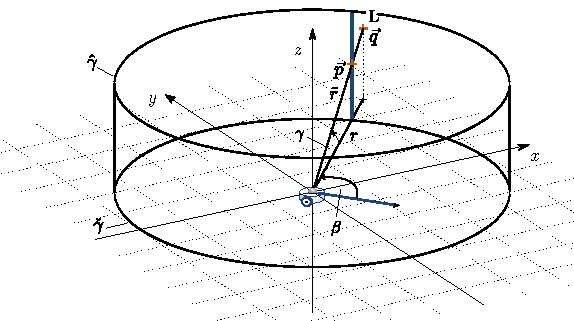
\includegraphics[width=0.975\textwidth]{media/cylinder_coordinates_simple.pdf}
  \end{center}
  \caption{Spherical coordinate system used throughout the algorithm. The projected position $\vec p$ of the landmark $L$ is given by the azimuthal angle $\beta$ and the elevation angle $\gamma$. The landmark position is given by $\beta, \gamma$ and the ground distance $r$.}
  \label{fig:cylinder_coordinates_simple}
\end{figure}

\begin{figure}[p]
  \begin{center}
   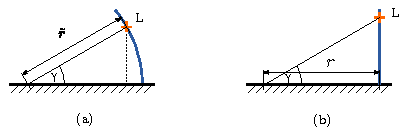
\includegraphics[width=0.8\textwidth]{media/hypot_vs_ground_distance.pdf}
  \end{center}
  \caption{Comparison between classical spherical coordinates (a) and the modified spherical coordinates (b). In (a), $\tilde r$ is measured as the distance between the coordinate-system origin and the landmark point $L$ (corresponds to the length of the hypotenuse in the above triangle). Landmarks with the same distance $\tilde r$ are thus assumed to be curved towards the camera (blue line). In the modified spherical coordinates depicted in (b), the distance $r$ is measured as the ground distance to the landmark. Consequently landmarks with the same distance $r$ shape a straight vertical line. As a side-effect, the elevation angle $\gamma$ is not of interest when a landmark point is $\vec q$ projected onto the $x$-$y$-plane. In contrast to classical spherical coordinates, points with $\gamma = \pm 90^\circ$ and $r = 0$ cannot be uniquely described in the modified spherical coordinates.}
  \label{fig:hypot_vs_ground_distance}
\end{figure}

\subsection{Assumptions}

\label{sec:assumptions}

The algorithm contains several idealizing assumptions, which may not be fully valid in a real-world environment. These assumptions cover both the robot and its environment.
\begin{enumerate}[(1)]
 \item \textit{Perfect path integration:} The robot is capable of perfect path integration and can thus (given an initial offset) determine its current world position and orientation at any time step. There is no mobile robot which completely fulfills this assertion without an external position reference \citep[chapter 3, ``Mobile Robot Kinematics'', p. 57ff]{AutonomousMobileRobots}. Yet the relative movement measured by the odometry over a short time window (as needed in the algorithm) and in ``normal'' operation (no wheel slippage) is assumed to be relatively error-free.
 \item \textit{Limited degrees of freedom:} It is assumed that the robot is only moving in the $x$-$y$-plane and only rotates around its $z$-axis. Neither is there any change in the elevation, nor does the robot tilt around any other axis. Those assumptions are likely to be violated in the real-world. Especially in outdoor environments the ground is never perfectly even and thus both changes in elevation and tilt can occur. In indoor environments e.g. carpets or thresholds are possible problems. We may assume that any tilting is removed from the input images in a preprocessing step, yet this is out of the scope of this thesis.
 \item \textit{Brightness constancy:} Neither are there changes in the global illumination (e.g. lights being switched on/off or the sun being covered by clouds) nor does the surface brightness change between the images. As pointed out by \cite{flowchapter05}, this ``brightness constancy'' only holds in environments containing surfaces without specularities (Lambertian surfaces), ``a distant point light source, no object rotations and no secondary illumination (shadows or inter-surface reflection)''. Yet this brightness constancy assumption (especially the lack of specularities) is used in most optical flow algorithms and seems to work remarkably well in practice.
 \item \textit{Static world:} The world is static, the robot is the only moving entity. This assumption may not be fulfilled in outdoor environments with vegetation and also in crowded indoor scenes. Moving objects may cause wrong depth reconstruction and thus cause false positive obstacles. Therefore the navigation algorithm which processes the obstacle points returned by the algorithm must be capable of discarding obstacles in its internal map that prove to be nonexistent.
\end{enumerate}
The robustness of the algorithm regarding violation of assumption (1) is explicitly tested in section \ref{sec:noise}.

\section{Depth reconstruction}

\label{sec:outline}

The goal of the \textit{depth reconstruction} stage is to estimate the ground distance $r$ for the landmarks corresponding to each pixel $\vec p = (\beta, \gamma)^T$ in the current view image $\img{CV}$. Consequently, the required result is a depth map $\img{R}(\vec p)$.

The general idea of the depth reconstruction is to exploit the parallax information present in the two images: Objects with a large distance only show a small displacement between the two images, whereas objects close to the camera show a relatively large displacement. This object displacement information is described by the motion field.

First a short introduction to optical flow estimation will be given. In conjunction with the motion parameters, the minimization problem underlying optical flow can then be reduced from a two-dimensional problem in each image point to a one dimensional problem. An approximative heuristic for this one dimensional problem is then given as minimum search in the so called \textit{error stack}.

\subsection{Short introduction to optical flow estimation}

When moving a camera in a static 3D-scene, the projected object points move along certain two-dimensional paths. These paths depend on the camera motion, the object distance and position in the projected image. The velocity of each pixel at position $x, y$ in the image and time $t$ is referred to as \textit{motion field} \citep{flowchapter05}. The motion field is a theoretical construct which can only be calculated if the camera parameters, camera motion and the exact position of each landmark point $\vec q$ are known.

Optical flow is an estimation of the motion field for a set of images $\img{I}_1$ and $\img{I}_2$ captured at discrete times $t_1$ and $t_2$ during the camera movement (in general optical flow may be estimated from more than two images). By definition, optical flow cannot express the motion of the underlying objects, but of the light intensities created by these objects \citep[][chapter 4.2.7 ``Motion and optical flow'', p. 189]{AutonomousMobileRobots}. The global optical flow estimation problem can generally be expressed as finding a vector field $\vec u : \R^2 \longrightarrow \R^2$ which minimizes the following error function \citep[adapted from][]{hornSchunck}:
\begin{equation}
  E(\vec u) = \int_{\vec p} \left( \|\img{I}_1(\vec p) - \img{I}_2(\vec p + \vec u(\vec p))\|_1 + \lambda \| \nabla \vec u(\vec p) \| \right) \; \mathrm{d}\vec p \label{eqn:optical_flow} \; .
\end{equation}
The first summand $\|\img{I}_1(\vec p) - \img{I}_2(\vec p + \vec u(\vec p))\|$ expresses the residual error after warping the second image according to the vector field. Note that minimization of this term is only valid due to assumptions (3) (brightness constancy) and (4) (static world).

The second term $\lambda \| \nabla \vec u(\vec p) \|$  enforces a certain ``smoothness'' to the vector field under the regularization parameter $\lambda$. This regularization is crucial for eliminating trivial solutions, such as simply mapping pixels with the same intensity to each other.

Although some approaches try to globally solve the minimization problem stated by equation \ref{eqn:optical_flow} \citep[e.g.][chapter 5 ``Real-time Optical Flow'']{totalVariation}, the solution presented here only minimizes the error for the local surroundings of each pixel in order to fulfill the real-time constraint on an embedded system.

\subsection{Motion field equation}

Given the motion parameters $d, \alpha, \psi$, the motion field could actually be calculated if the distance to each landmark point $\img{R}(\vec p)$ was known:

Let $\vec q = (x, y, z)^T$ be the position of a landmark $L$ in robot coordinates (origin at the robot center, $x$-axis aligned with the robot orientation). The projection $P : \R^3 \longrightarrow \R^2 $ that projects $\vec q$ onto $\vec p = (\beta, \gamma)^T$ in the image plane is given as:
\begin{equation}
 \vec p = P(\vec q) = \begmat \beta \\ \gamma \finmat = \begmat
  \atantwo(y, x) \\
  \arctan\left(\frac{z}{\sqrt{x^2 + y^2}}\right)
 \finmat
 \label{eqn:project}
\end{equation}
The inverse $P^{-1} : \R^2 \longrightarrow \R^3$ with free parameter $r$ (ground distance) is given as:
\begin{equation}
 \vec q = P^{-1}(\vec p; r) = \begmat x \\ y \\ z \finmat = r \cdot \begmat
  \cos(\beta) \\
  \sin(\beta) \\
  \tan(\gamma)
 \finmat
 \label{eqn:unproject}
\end{equation}
The motion vector $\vec u(\vec p; T, r)$ describing the relative movement of a pixel at position $\vec p$ between the current view and the snapshot image can now be calculated as
\begin{equation}
 \vec u(\vec p; T, r) = P(T \cdot h(P^{-1}(\vec p; r))) - \vec p \label{eqn:motion_field_vector}
\end{equation}
where $T \in \R^{3 \times 4}$ is a homogeneous transformation matrix expressing the robot movement between $\img{CV}$ and $\img{SS}$ in world coordinates:
\begin{equation}
 T = T(d, \alpha, \psi) = \begmat
   \cos(\psi) & \sin(\psi) & 0 & d \cdot \cos(\alpha) \\
  -\sin(\psi) & \cos(\psi) & 0 & d \cdot \sin(\alpha) \\
 0 & 0 & 1 & 0
 \finmat
 \label{eqn:transform}
\end{equation}
The sole purpose of the mapping $h : \R^3 \longrightarrow \R^4$ is to transform three dimensional points to homogeneous coordinates. $h$ is defined as $(x, y, z)^T \mapsto (x, y, z, 1)^T$. See figure \ref{fig:cylinder_coordinates_transformation} for an interpretation of the motion field vectors.

\begin{figure}[t]
 \begin{center}
  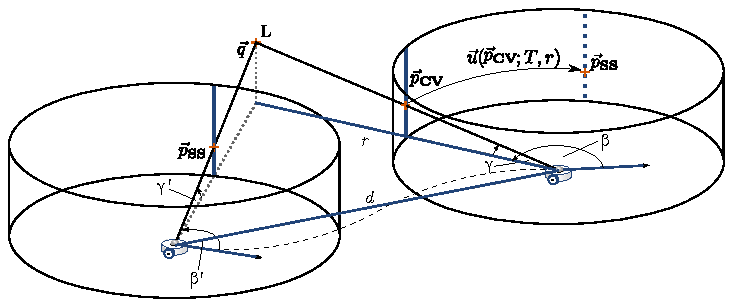
\includegraphics[width=0.975\textwidth]{media/cylinder_coordinates_transformation.pdf}
 \end{center}
 \caption{The motion field equation can be interpreted as follows: Given a point $\vec p_{\img{CV}} = (\beta, \gamma)^T$ in $\img{CV}$ (right), the motion field vector $\vec u(\vec p_{\img{CV}}; T, r)$ predicts the position $\vec p_{\img{SS}} = (\beta', \gamma') = \vec u(\vec p_{\img{CV}}; T, r) + \vec p_{\img{CV}}$ in which the same landmark point $L$ would be visible in $\img{SS}$ (right) under the assumption that $L$ has the distance $r$.
}
 \label{fig:cylinder_coordinates_transformation}
\end{figure}

\subsection{Flow parametrization}

By combining equation \ref{eqn:motion_field_vector} from above and the error function in equation \ref{eqn:optical_flow}, the minimum search can be reduced from a two-dimensional problem in each pixel (finding an arbitrary flow vector $\vec u$) to a one dimensional optimization problem (finding the best matching depth value $r$ for each pixel):
\begin{equation}
 E(\img{R}) = \int_{\vec p} \left( \|\img{I}_1(\vec p) - \img{I}_2(\vec p + \vec u(\vec p;  T, \img{R}(\vec p)))\|_1 + \lambda \nabla \| \vec u(\vec p; T, \img{R}(\vec p)) \| \right) \;\mathrm{d}\vec p\label{eqn:parametrized_optical_flow}
\end{equation}
Hence the depth field $\img{R}(\vec p)$ can be seen as an implicit characterization of the optical flow field under the motion parameters $d, \alpha$ and $\psi$. Note that these parameters are only known if assumption (1) (perfect path integration, see section \ref{sec:assumptions}) is valid --- otherwise the motion field cannot be predicted.

\subsection{Error stack calculation}

\label{sec:error_stack}

The heuristic used in this approach searches local minima in the so called \textit{error stack} $\img{E}$ in order to estimate the depth field $\img{R}(\vec p)$. Each of the $n$ layers $\img{E}_i$ contains the residual error (first summand in equation \ref{eqn:parametrized_optical_flow}) evaluated for a constant depth $r_i$:
\begin{equation}
 \img{E}_i(\vec p) = \|\img{CV}(\vec p) - \img{SS}(\vec p + \vec u(\vec p; T, r_i))\|_1 \text{ where }  0 \leq i < n \label{eqn:error_stack_layer}
\end{equation}
Figuratively speaking, this equation is equivalent to first calculating a warped snapshot image $\img{SS'}_i$, that predicts ``what the current view would look like'' under the assumption that all image points had the same distance $r_i$. The residual error stored in each error stack layer is then given as $\img{E}_i = \| \img{CV} - \img{SS'}_i \|_1$. See figure \ref{fig:error_stack} for an example.

Note that some source pixel coordinates may not be in range when calculating the warped snapshot. The error value stored for the target pixel in the error stack layer should then be set to a large value (see figure \ref{fig:error_stack}).

\paragraph{Conventions for the distance series:} The $r_i$ are left open at this point, yet (by convention) any choice has to meet the following conditions:
\begin{enumerate}[1.]
 \item The series $r_i$ is strictly monotonically decreasing.
 \item $r_0 = \infty$ (for $i = 0$ the motion vector length should equal zero for all pixels).
 \item The step from $r_i$ to $r_{i + 1}$ should increase the maximum horizontal flow vector length by one pixel. This way the pixels in $\img{SS'}_i$ are at most shifted by one pixel in horizontal direction between two error stack layers, which allows to exploit the complete horizontal image resolution in the error stack calculation.
 \item $r_{n - 1}$ should be chosen near the smallest possible distance between an obstacle and the camera.
 \item There has to be some strictly monotonically decreasing, continuous function $r(j) : \R^+ \longrightarrow \R^+$, where $r(i) = r_i$ for all $i$.
\end{enumerate}
A concrete choice for the $r_i$ is presented in section \ref{sec:index_to_depth}.

\paragraph{Index related error function:} Combining the error stack equation (\ref{eqn:error_stack_layer}) and the parametrized optical flow equation (\ref{eqn:parametrized_optical_flow}) yields a minimization of the \textit{index field} $\img{J}(\vec p)$, that describes the error stack index chosen for each pixel:
\begin{align}
 E(\img{J}) &= \int_{\vec p} \left( \img{E}_{\img{J}(\vec p)}(\vec p) + \lambda \| \nabla \vec u(\vec p; T, r(\img{J}(\vec p))) \| \right) \; \mathrm{d}\vec p \nonumber \\
 &\approx \int_{\vec p} \left( \img{E}_{\img{J}(\vec p)}(\vec p) + \lambda \| \nabla \img{J}(\vec p) \| \right) \; \mathrm{d}\vec p \label{eqn:global_min_index}
\end{align}

At first glance $\nabla \vec u(\vec p; T, r({\img{J}(\vec p))}) \approx \nabla \img{J}(\vec p)$ seems to be a very rough approximation, yet due to the conventions presented above, the error stack index $i$ is approximately proportional to the flow vector length. Consequently a smooth index field $\img{J}(\vec p)$ implies a smooth flow vector field $\vec u(\vec p; T, r({\img{J}(\vec p))})$.

\begin{figure}[p]
 \centering
 \begin{footnotesize}
 \begin{tabular}{m{0.025\textwidth} m{0.575\textwidth} m{0.4\textwidth}}
  (a) & 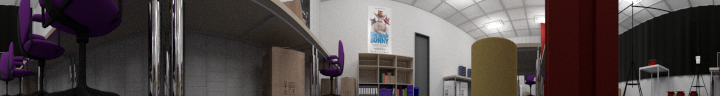
\includegraphics[width=0.55\textwidth]{media/warped/cv.png} & $\img{CV}$ (current view image) \\
  (b) & 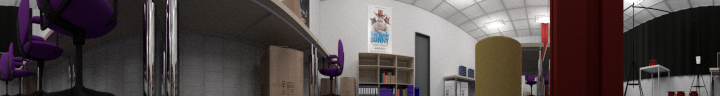
\includegraphics[width=0.55\textwidth]{media/warped/ss.png} & $\img{SS}$ (snapshot image) \\
  (c) & 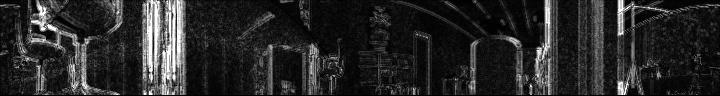
\includegraphics[width=0.55\textwidth]{media/warped/warped_depth_0.png} & $\img{E}_1$ with $r_1 = \infty$ \\
  (d) & 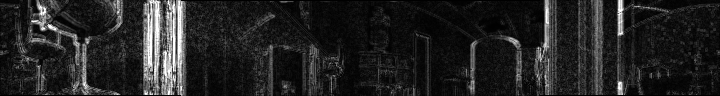
\includegraphics[width=0.55\textwidth]{media/warped/warped_depth_1.png} & $\img{E}_2$ with $r_2 = 4.58 \, \mathrm{m}$ \\
  (e) & 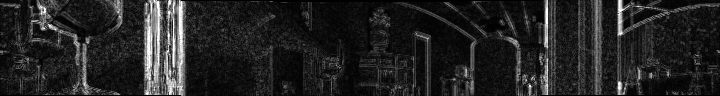
\includegraphics[width=0.55\textwidth]{media/warped/warped_depth_2.png} & $\img{E}_3$ with $r_3 = 2.29 \, \mathrm{m}$ \\
  (f) & 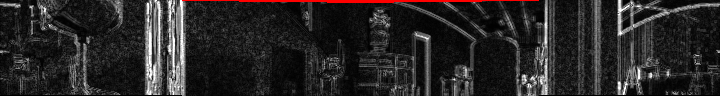
\includegraphics[width=0.55\textwidth]{media/warped/warped_depth_3.png} & $\img{E}_4$ with $r_4 = 1.15 \, \mathrm{m}$ \\
  (g) & 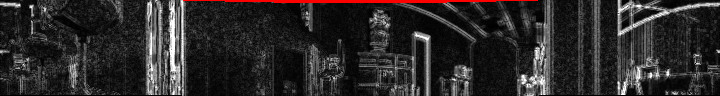
\includegraphics[width=0.55\textwidth]{media/warped/warped_depth_4.png} & $\img{E}_5$ with $r_5 = 0.92 \, \mathrm{m}$ \\
  (h) & 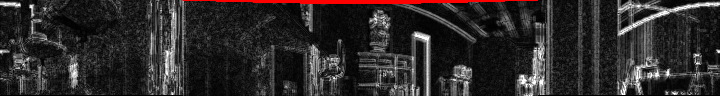
\includegraphics[width=0.55\textwidth]{media/warped/warped_depth_5.png} & $\img{E}_6$ with $r_6 = 0.76 \, \mathrm{m}$ \\
  (i) & 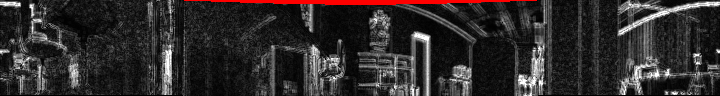
\includegraphics[width=0.55\textwidth]{media/warped/warped_depth_6.png} & $\img{E}_{15}$ with $r_{15} = 0.31 \, \mathrm{m}$
 \end{tabular}
 \end{footnotesize}
 \caption{Visualization of a series of error stack layers. The error stack layers shown in the images (c) to (i) were calculated for the current view and snapshot shown in (a) and (b) (the original input images are monochrome). The brightness of the pixels in the error stack images corresponds to the error value. Note how certain objects ``disappear'' (have only a small error) in certain error stack images, like the silhouettes of the yellow cylinder in $\img{E}_5$ or the table legs in $\img{E}_6$, while the error for distant objects like the door frame increases with each layer. The image regions marked red form those for which no prediction can be made and thus have an infinite error.}
 \label{fig:error_stack}
\end{figure}

\subsection{Input image augmentation}

\label{sec:preprocessing}

\begin{figure}[p]
	\centering
	\subbottom[Monochrome image]{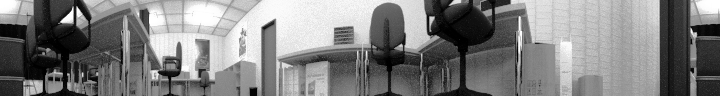
\includegraphics[width=0.75\textwidth]{media/gradient/in_brightness.png}}
%	\subbottom[$x$-derivative]{\includegraphics[scale=0.248]{media/gradient/in_derivative_x.png}}
%	\subbottom[$y$-derivative]{\includegraphics[scale=0.248]{media/gradient/in_derivative_y.png}} \\
	\subbottom[Combined pseudocolor image]{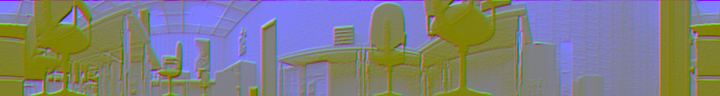
\includegraphics[width=0.75\textwidth]{media/gradient/out.png}}
	\caption{Comparison between the original monochrome image and the pseudo-color image resulting from the transformation described in equation \ref{eqn:dimensionality_increase}. The brightness is mapped to the blue channel, $x$- and $y$-derivatives to the red and green channels, respectively.}
	\label{fig:pseudocolor_image}
\end{figure}

Comparing individual pixels from a monochrome image $\img{I}$ (as in the error stack equation \ref{eqn:error_stack_layer}) discards all spatial information that is encoded in the environment of each pixel.

In order to increase the information contained within a single pixel, one can increase its dimensionality. In the resulting feature space, each pixel can be seen as a local feature descriptor. The augmentation proposed here adds the image gradients in horizontal and vertical direction as a second and third component to each pixel, leading to the following equation for the augmented image $\img{\tilde I}$:
\begin{equation}
	\img{\tilde I}(\vec p) = \begmat
		\img{I}(\vec p),
		\left. \frac{\partial \img{I}}{\partial x \vphantom{y}} \right|_{\vec p},
		\left. \frac{\partial \img{I}}{\partial y} \right|_{\vec p}
	\finmat^T
	\label{eqn:dimensionality_increase}
\end{equation}
As a drawback, this augmentation reduces the overall spatial resolution: Estimating the derivative on discrete images (e.g. using the $3 \times 3$ Sobel kernel) incorporates at least three pixels. Moreover, the derivation increases the image noise \citep[][p. 200]{AutonomousMobileRobots}.

Figure \ref{fig:pseudocolor_image} shows the result of equation \ref{eqn:dimensionality_increase} being applied to an input image. Note how the image edges (representing the regions with the largest gradient) are prominently marked in the resulting image. Thus ``a sense of edges'' is added to the algorithm.

\subsection{Minimum error search}

\label{sec:minimum_error_search}
As stated in equation \ref{eqn:global_min_index}, estimating depth and optical flow is a matter of minimizing the global error by choosing appropriate error stack indices $\img{J}(\vec p)$ for each pixel $\vec p$. A na\"{\i}ve heuristic to estimating depth for each pixel would be to simply select the error stack layer that holds the global minimum error for each pixel:
\begin{equation}
	\img{J}(\vec p) = \arg \min_{i} \img{E}_i(\vec p) \label{eqn:naive_minimum_search}
\end{equation}
However, while being very simple to compute, this heuristic has a severe disadvantage: Computing the index without regarding neighboring pixels completely disregards the smoothness term. Additionally, as the error stack may not have a single pronounced minimum but multiple local minima with very small difference, the result is prone to noise.

Assuming that most objects cover more than a single pixel in the image and neighboring pixels have approximately the same distance, we can modify equation $\ref{eqn:naive_minimum_search}$ to respect the surroundings of each pixel. Let $W_{\vec p}$ be a (possibly space-variant) two-dimensional filter kernel with radius $r_W$:
\begin{equation}
	\img{J}(\vec p) = \arg \min_{i} \left( \img{E}_i \ast W_{\vec p} \right)_{\vec p} \label{eqn:kernel_minimum_search}
\end{equation}
The matrix $W_{\vec p}$ is subsequently called \textit{error propagation matrix} as it ``propagates'' error values from neighboring pixels to its center pixel.

In large homogeneous image regions where multiple error stack layers contain very small error values (see the wall regions in figure \ref{fig:error_stack}), depth cannot be reconstructed (at least not without using global approaches) and equation \ref{eqn:kernel_minimum_search} will very likely produce noise in such regions. In a later step, this noise might produce unwanted false obstacle points. Adding a linear bias $\tau \cdot i$ to the error function allows to classify homogeneous image regions  as ``very distant'', in which case they do not hinder the obstacle detection:
\begin{equation}
	\img{J}(\vec p) = \arg \min_{i} \left( \left( \img{E}_i \ast W_{\vec p} \right)_{\vec p} + \tau \cdot i \right) \label{eqn:kernel_minimum_search_bias}
\end{equation}

\paragraph{Choices for $W_{\vec p}$:} Simple space-invariant choices for $W_{\vec p} = W$ include a matrix of ones or a Gaussian filter kernel. A space-variant filter kernel $W_{\vec p}$ which takes object boundaries into account and thus only propagates error values for pixels belonging to the same object is presented in appendix \ref{sec:kernels}.

\subsection{Minimum error refinement}

\label{sec:index_field_refinement}

\begin{figure}[t]
 \begin{center}
  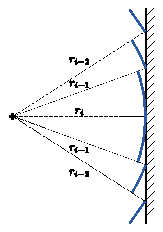
\includegraphics[width=0.35\textwidth]{media/discrete_indices_artifacts.pdf}
 \end{center}
 \caption{Local map (top-down view) showing the artifacts created by approximating a planar surface with a set of circles having discrete radii (blue).}
 \label{fig:discrete_indices_artifacts}
\end{figure}

% \begin{figure}[p]
%  \begin{center}
%    \includegraphics[width=0.975\textwidth]{media/minimum_error_search.pdf}
%   \end{center}
%   \caption{Visualization of the minimum error search in the error stack layers. For each pixel $\vec p$ the minimum error is searched within a region specified by the filter kernel $W_{\vec p}$. The discrete minimum index $\img{J}(\vec p)$ is then refined by searching the minimum $\img{\tilde J}(\vec p)$ in the piecewise error stack approximations plus a regularization term. The piecewise error stack approximations are indicated by the dashed blue lines in the image.}
%   \label{fig:minimum_error_search}
% \end{figure}

Equation $\ref{eqn:kernel_minimum_search}$ produces an index field $\img{J}(\vec p)$ consisting of discrete values. This is especially problematic if a planar surface needs to be reconstructed (see figure \ref{fig:discrete_indices_artifacts}). Additionally, the discontinuity causes a high penalty in the smoothness term of the global error equation \ref{eqn:optical_flow}. In this section the initial index field $\img{J}(\vec p)$ as defined in equation $\ref{eqn:kernel_minimum_search_bias}$ will be refined (allowing non-discrete solutions) and regularized (addressing the smoothness term) which leads to the final index field $\img{\tilde J}(\vec p)$.

\paragraph{Refinement:} The discontinuity problem can be solved by approximating the error stack in each layer $i$ and pixel $\vec p$ utilizing piecewise polynomials of second degree (quadratic; allows for trivial analytical solution), resulting in a set of functions $\tilde E_{i}(j; \vec p)$ with the following properties:
\begin{equation*}
	\begin{aligned}
		\tilde E_{i}(j; \vec p) &:= \begmat j^2 & j & 1 \finmat \cdot \vec w \\
		\tilde E_{i}(i + j; \vec p) &\overset{!}= \img{E}_{i + j}(\vec p) + \tau \cdot (i + j)\quad \forall \quad j \in \{-1, 0, 1\}
	\end{aligned}
\end{equation*}
Solving this set of linear equations yields the following weight vector $\vec w$:
\begin{equation}
	\vec w = \begmat w_2 \\ w_1 \\ w_0 \finmat =
	\begmat
		\frac{1}2 & -1 & \frac{1}2 \\
		-i - \frac{1}2 & 2 i & -i + \frac{1}2 \\
		\frac{1}2(i^2 + i) & -i^2 + 1 & \frac{1}2 (i^2 - i)
	\finmat
	\cdot
	\begmat
		\mathbf{E}_{i - 1}(\vec p) + \tau \cdot (i - 1) \\
		\mathbf{E}_{i}(\vec p) + \tau \cdot i \\
		\mathbf{E}_{i + 1}(\vec p) + \tau \cdot (i + 1)
	\finmat
	\label{eqn:polynomial_coeffs}
\end{equation}
If one of the error layers $\mathbf{E}_{i - 1}$ or $\mathbf{E}_{i + 1}$ does not exist, a linear approximation is chosen instead.

\paragraph{Regularization:} The regularization term penalizes large variances in the index field. For a single reference point $\vec q$, the quadratic regularization function $R(j; \vec q)$ is given as a polynomial
  $$R(j; \vec q) = \lambda \cdot (\img{J}(\vec q) - j)^2$$
which quadratically increases the penalty according to the difference between the index $j$ in the current point $\vec p$ and the index of the reference point $\vec q$.

\paragraph{Final minimization formula:} Again the error function is not minimized for every individual pixel, but for a weighted region surrounding each pixel as defined by the convolution kernel $W_{\vec p}$. For compact notation, let $A(\vec p) := \{\vec p + (\beta(x), \gamma(y))^T \mid -m \leq x, y \leq m\}$ denote the pixel coordinates beneath the convolution window at position $\vec p$ and let $\omega_{\vec p}^{\vec q}$ for $\vec q \in A(\vec p)$ denote the corresponding value in the convolution matrix $W_{\vec p}$. The refinement of the initial (integral) index field $\img{J}$, leading to the refined, real-valued index field $\img{\tilde J}$, is then given as
\begin{equation}
 \img{\tilde J}(\vec p) = \argmin_{\img{J}(\vec p) - 1 \leq j \leq \img{J}(\vec p) + 1} \sum_{\vec q \in A(\vec p)} \omega_{\vec p}^{\vec q} \cdot \left(\tilde E_{\img{J}(\vec p)}(j; \vec q) + R(j; \vec q) \right)
 \label{eqn:index_field_refinement}
\end{equation}
As the sum only contains quadratic polynomials, the minimum can be calculated analytically.

Note that the refinement step can be repeated multiple times. The indices in $\img{\tilde J}(\vec p)$ are then rounded to the nearest integers and treated as the initial index field $\img{J}(\vec p)$.

Once the final index map $\img{\tilde J}(\vec p)$ has been built, the index-to-depth function $r(j)$ can be used to obtain the desired depth map:
  $$\img{R}(\vec p) = r(\img{\tilde J}(\vec p))$$


\section{Obstacle detection}

The simple heuristic used in the depth reconstruction was designed for fast evaluation and does by no means guarantee to find a perfect depth estimation. Additionally, noise in the images or the motion parameters $d, \alpha, \psi$ (and thus a violation of the assumptions presented in section \ref{sec:assumptions}) inevitably leads to noise in the depth map.

For obstacle detection, a local environment map (top-down projection onto the $x$-$y$-plane) of the reconstructed landmark points is created. The aim of this map is to improve the depth reconstruction result by combining depth maps resulting from multiple depth reconstruction steps. It then allows the selection of actual obstacle points which form the result of the overall algorithm.

\subsection{Probabilistic landmark model}

\label{sec:prob_landmarks}

\begin{figure}[p]
 \begin{center}
  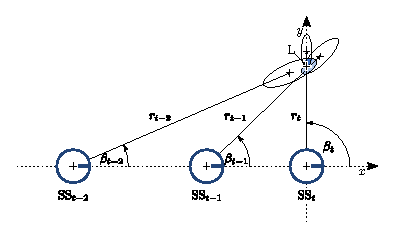
\includegraphics[width=0.82\textwidth]{media/obstacle_map_jitter.pdf}
 \end{center}
 \caption{The Gaussian distributions for reconstructed landmark positions from multiple time steps can overlap in such a way that their sum forms a distinct maximum at (or at least near) the actual landmark position $L$. Consequently, whenever a value above a certain threshold appears in the map, the underlying point is emitted as an obstacle. Note that the sum of two overlapping (corresponding to the intersection of certain contour lines) Gaussian distributions does not necessarily yield a maximum at the landmark position as suggested by the drawing. Yet the distributions used in this approach have a relatively high distance variance $\sigma_r$ in comparison to their direction variance $\sigma_\beta$. Thus overlapping Gaussians implicitly triangulate the landmark and a maximum is probable.}
 \label{fig:obstacle_map_jitter}
\end{figure}

\begin{figure}[p]
 \begin{center}
  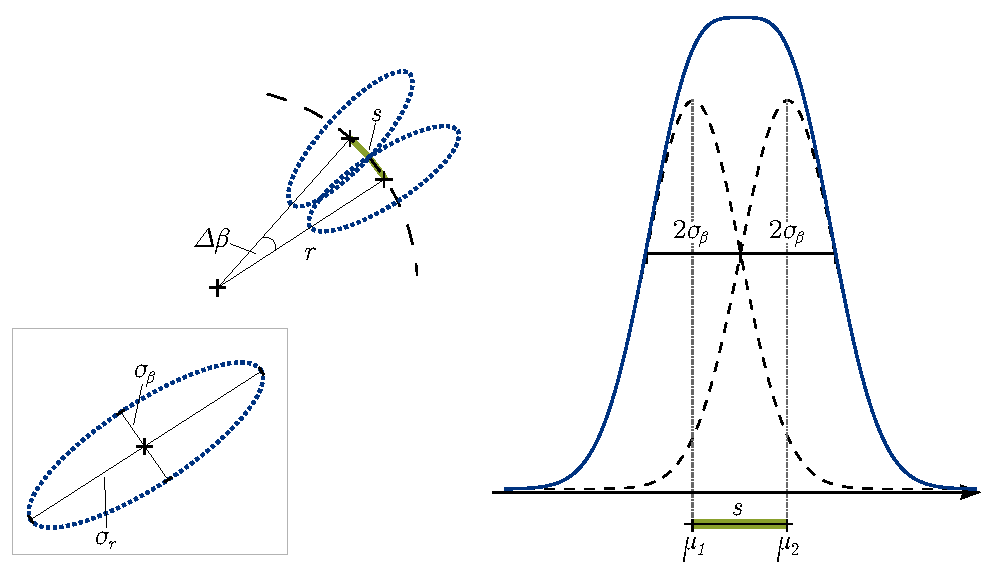
\includegraphics[width=0.91\textwidth]{media/sigma_beta.pdf}
 \end{center}
 \caption{Calculation of the variance $\sigma_\beta$. Adjacent Gaussian distributions with the same radius $r$ should form a nearly uniform distribution between $\mu_1$ and $\mu_2$. See also appendix \ref{proof:sigma_beta}.}
 \label{fig:sigma_beta}
\end{figure}

The reconstructed landmark points $(\beta, \gamma, r)^T$ can be projected onto the $x$-$y$-plane by just omitting the $\gamma$ angle, as $r$ was chosen as the ground distance (see section \ref{sec:panoramic_coordinates} and the corresponding figure \ref{fig:hypot_vs_ground_distance}). The projected landmark point $\vec q$ is hence specified by the polar coordinates $\vec q = (\beta, r)^T$.

As stated above, the \textit{estimated} landmark position $\vec q_E$ as returned from the depth reconstruction is prone to noise. Assume a Gaussian distribution with mean at $\vec q_E$ for the probability of the \textit{real} landmark position $\vec q_R$:
\begin{equation}
  \vec q_R \sim \mathcal{N}\left(\vec q_E, \Sigma(\vec q_E) \right) \text{ where } \Sigma(\beta, r) := \begmat \sigma_\beta^2 & 0 \\ 0 & \sigma_r^2 \finmat
  \label{eqn:gaussian_polar}
\end{equation}
Let $\mathcal{C} : (\beta, r)^T \mapsto r \cdot (\cos(\beta), \sin(\beta))^T$ denote the transformation from polar to Cartesian coordinates. As an approximation, equation \ref{eqn:gaussian_polar} can be written for Cartesian coordinates as:
\begin{equation}
  \mathcal{C}(\vec q_R) \sim \mathcal{N}\left(\mathcal{C}(\vec q_E), \Sigma_{\mathcal{C}}(\vec q_E)\right)
\end{equation}
where $\Sigma_{\mathcal{C}}$ is the corresponding covariance matrix in Cartesian space given as (see \ref{proof:covariance_matrix_transformation} for the derivation):
\begin{equation}
  \Sigma_{\mathcal{C}}(\beta, r) = \begmat
    (\sigma_r \cos(\beta))^2 + (r \sigma_\beta \sin(\beta))^2 & \cos(\beta) \sin(\beta) (\sigma_r^2 - (r \sigma_\beta)^2) \\
    \cos(\beta) \sin(\beta) (\sigma_r^2 - (r \sigma_\beta)^2) & (\sigma_r \sin(\beta))^2 + (r \sigma_\beta \cos(\beta))^2
  \finmat
  \label{eqn:cartesian_covariance}
\end{equation}


\paragraph{Derivation of the distribution variances:} Until now the variances in  direction $\sigma_\beta$ and in distance $\sigma_r$ were left open.

The distance variance $\sigma_r$ depends on the choice of the yet unknown index-to-depth function $r(j)$ and will be introduced along with the concrete choice in section \ref{sec:index_to_depth}.

However, $\sigma_\beta$ only depends on the horizontal image resolution $\Delta \beta := \nicefrac{2\pi}w$ and can be derived by demanding that two adjacent Gaussian distributions (with $| \beta_1 - \beta_2 | = \Delta \beta$) should overlap in such a way that their sum forms a near-uniform distribution in the region between $\beta_1$ and $\beta_2$. This choice is motivated by the fact that the probability of an obstacle point being located somewhere between two image columns $\beta_1$ and $\beta_2$ is the same as the probability of an obstacle point being located exactly on a certain image column $\beta$.

One can show (see appendix \ref{proof:sigma_beta}) that $\sigma_\beta$ is now given as
\begin{equation}
 \sigma_\beta = \frac{\Delta \beta}2 = \frac{\pi}{w}
 \label{eqn:sigma_beta} \; .
\end{equation}
Multiplying $\sigma_\beta$ with $r$ produces the Cartesian equivalent of the angular variance, as $\Delta \beta \cdot r$ denotes the length $s$ of the curve segment between $\beta_1$ and $\beta_2$ (see figure \ref{fig:sigma_beta}).

\subsection{Distribution accumulation and obstacle detection}

\label{sec:obstacle_detection}

It is hoped that the accumulated Gaussian distributions (forming the so called \textit{density values}) resulting from subsequent depth reconstruction steps produce pronounced maxima at the real landmark positions. This is possible as the probability distributions have rather small variance in angular direction, but a relatively large variance in distance direction. Thus intersecting Gaussian distributions implicitly triangulate the result (see figure \ref{fig:obstacle_map_jitter}).

Let $\img{M}$ be a discrete Cartesian map matrix that spans a region of $2 \cdot r_M \times 2 \cdot r_M$ meters (where $r_M$ is radius of the map), and let the origin $\img{M}(0, 0)$ correspond to the center of the map matrix. The obstacle detection algorithm is given as follows:

\paragraph{Map position update:} Rotate and shift the map matrix such that the camera is always located at the map origin and the angle $\beta = 0$ is always relative to the current translatory motion direction $\alpha$.

\paragraph{Map decay:} In order to ensure the locality of the map, all old density values are multiplied with a decay factor $\delta$ depending on the translatory distance $d$:
\begin{equation}
 \img{M}(x, y) \gets \img{M}(x, y) \cdot \delta \; \forall \; x, y \text{ where } \delta = \exp(-\epsilon \cdot d) \; .
 \label{eqn:map_decay}
\end{equation}
The free parameter $\epsilon$ is used as a conversion factor between $d$ and $\delta$. This way old density values are gradually discarded from the map as the robot moves through the world.

\paragraph{Distribution accumulation:} For each reconstructed and projected landmark point $\vec q_k = (\beta_k, r_k) \in Q$ the corresponding probability distributions are accumulated and added to the old density values in the discrete map:
\begin{equation}
 \img{M}(x, y) \gets \img{M}(x, y) + \sum_{\vec q \in Q} \mathcal{N}\left((x, y)^T \mid \mathcal{C}(\vec q), \Sigma_{\mathcal{C}}(\vec q)  \right) \; \forall \; x, y
\end{equation}

\paragraph{Obstacle detection:}

\begin{figure}[t]
 \begin{center}
  \subbottom[Color coded local environment map]{
    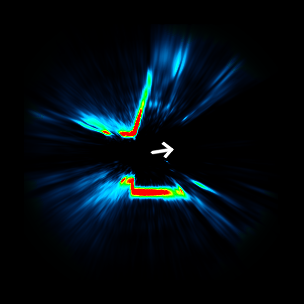
\includegraphics[width=0.3\textwidth]{media/local_obstacle_map_2.png}
  }
  \subbottom[Thresholded map]{
    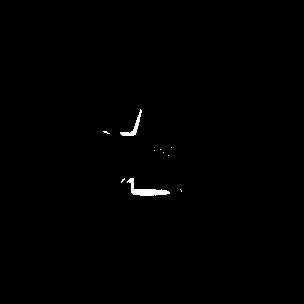
\includegraphics[width=0.3\textwidth]{media/local_obstacle_map_segmented.png}
  }
  \subbottom[Resulting obstacle points (orange)]{
    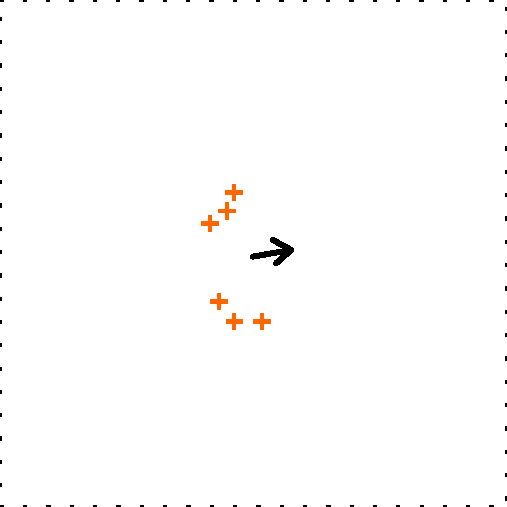
\includegraphics[width=0.3\textwidth]{media/local_obstacle_map_obstacles.pdf}
  }
 \end{center}
 \caption{Overview of the obstacle detection process. (a) shows a color coded environment map $\img{M}$ (black and blue correspond to small, green and yellow to medium and red to high density values), (b) shows the thresholded map $\img{\tilde M}$ and (c) the resulting obstacle points which form the result of the algorithm. The arrows in (a) and (c) indicate the robot orientation.}
 \label{fig:obstacle_map_process}
\end{figure}

If multiple distributions overlap in such a way that a distinct maximum is formed in the obstacle map, it is likely for this maximum to correspond to an actual landmark point. As outlined in figure \ref{fig:obstacle_map_process}, these distinct maxima are detected by generating a thresholded map
  $$\img{\tilde M}(x, y) \gets \begin{cases}
                              1 & \img{M}(x, y) > \eta \\
                              0 & \text{otherwise}
                             \end{cases} \quad \forall \; x, y$$
where $\eta$ is the threshold value. In a subsequent step, 4-connected components in $\img{\tilde M}$ are detected \citep[using the one-pass algorithm presented in][]{wiki:connected_component}. If they exceed a certain minimum size their centroid is returned as an obstacle point.

\paragraph{Obstacle point fragmentation and occupancy map:} As an extension to the above, large connected components are fragmented into multiple obstacle points. This is accomplished by dividing each connected component into square grid cells, counting the pixels in each cell and --- if a threshold is exceeded --- returning the centroid of the pixels in each grid cell as an obstacle point.

In order to prevent the algorithm from repeatedly returning the same obstacle points, obstacles are marked in a low resolution \textit{occupancy map} $\img{M_O}$. The size of $\img{M_O}$ is chosen in such a way that each pixel corresponds to one of the square grid cells mentioned above. The map position update is also applied to $\img{M_O}$ and obstacles at positions marked as occupied in $\img{M_O}$ are not returned.
